\begin{frame}{Implementacja algorytmu genetycznego}
    \begin{enumerate}
        \item \textbf{Osobniki} \\
        {\small Ciągi wag w postaci tablic liczb całkowitych.}
        % {\centering 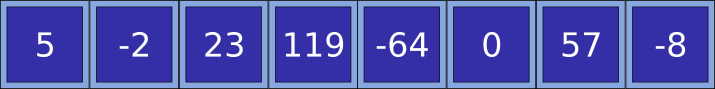
\includegraphics[width=6cm]{figures/genetyk_osobnik.png}}
        \item \textbf{Ewaluacja} \\
        {\small Pojedynek każdy-z-każdym (białe/czarne i na odwrót)}
        \item \textbf{Selekcja} \\
        {\small Ruletka (lepiej grające osobniki mają większą szansę na przejście).}
        \item \textbf{Krzyżowanie} \\
        {\small Dzieci powstają poprzez wymieszanie cech rodziców.}
        % {\centering 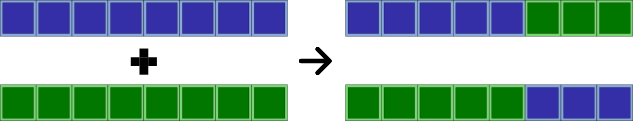
\includegraphics[width=6cm]{figures/genetyk_krzyzowanie.png}}
        \item \textbf{Mutacje} \\
        {\small Szansa na wylosowanie nowej wartości losowej wagi w ciągu.}
    \end{enumerate}

    \begin{columns}
		\begin{column}{.5\hsize}
			{\centering
			\begin{figure}
				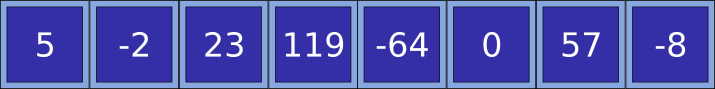
\includegraphics[width=5cm]{figures/genetyk_osobnik.png}
				\caption{Model poglądowy osobnika}
			\end{figure}
			}
		\end{column}
		\begin{column}{.5\hsize}
			{\centering
			\begin{figure}
				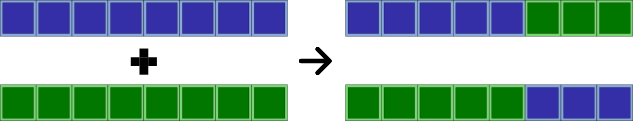
\includegraphics[width=5cm]{figures/genetyk_krzyzowanie.png}
				\caption{Model krzyżowania}
			\end{figure}
			}
		\end{column}
	\end{columns}
\end{frame}
